\documentclass{beamer}
\usepackage[english]{babel}
\usepackage[T1]{fontenc}
\usepackage[latin1]{inputenc}
\usetheme{Berlin}
\usecolortheme{rose}
\usepackage{lmodern}
\usepackage{mathtools,amssymb,mathrsfs,amsthm,amsmath,graphicx,float}
\graphicspath{{figures/}}

\newcommand{\p}{\mathbb{P}}

\title{\sc \bf Training Convolutional Networks \\with Noisy labels}
\subtitle{\tiny Sainbayar Sukhbaatar, Joan Bruna, Manohar Paluri, Lubomir Bourdev, and Rob Fergus - arXiv:1406.2080}
\author{\bf Maha ELBAYAD}
\institute{M2 MVA 2015/2016}
\date{\today}

\begin{document}

\begin{frame}
    \titlepage
\end{frame}
\section{Motivation}    
\begin{frame}[label=Motivation]
    \frametitle{Motivation}
    \begin{itemize}
    \item The performance of CNN depends on the amount of labeled samples and their presumable quality.
    \item Hand labelling is impractical $\rightarrow$ Shift to semi-automatic labelling - prone to inaccuracy and subjectivity.
    \pause
    \item Propose a generic way to handle two types of label noise:
    \begin{enumerate}
    \item Label flips\\
    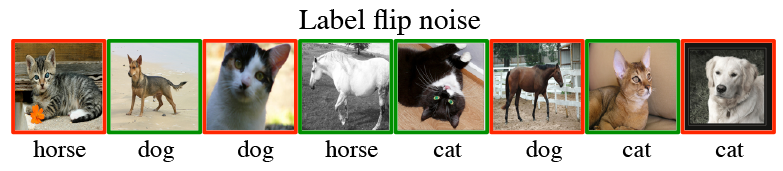
\includegraphics[width=6cm]{flip}
    \item Outliers\\
    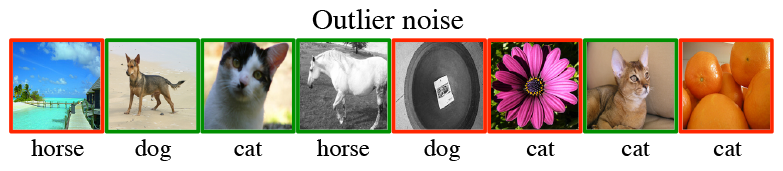
\includegraphics[width=6cm]{outlier}
    \end{enumerate}
    \end{itemize}
    
\end{frame}
    
\begin{frame}
    
    \frametitle{The Model}
    \framesubtitle{Noise modelling}
    Given a sample of labelled images $\mathcal I={(x_n,y_n)}_n$ where $y_n$ is the true label.\\
    Define noisy label distrbution:
    \[\p(\tilde y=i|y=j)=q_{i,k}\tag{A confusion matrix}\]
    Link the true label to the noisy label.
    \[\p(\tilde y|x,\theta,Q)=\sum_iq_{j,i}\p(y=i|x,\theta)\]
\end{frame}

\begin{frame}    
    \frametitle{The base model}
    


    
\end{frame}
    
\end{document}
